\documentclass[12pt]{article}

\usepackage[margin=1in]{geometry}
\usepackage{amsmath,amssymb,amsthm,mathtools}
\usepackage{enumitem}
\usepackage{tikz}
\usetikzlibrary{automata,positioning,arrows.meta}

\title{Granular Notes and Solutions for Sipser Chapter 1\\
Exercises 1.19, 1.20(e--h), and 1.29(b)}
\author{Wesley Weaver}
\date{\today}

\newcommand{\sipser}[1]{\footnote{Sipser, \emph{Introduction to the Theory of Computation}, 3rd ed., #1.}}

\begin{document}
\maketitle

\section*{How to use these notes}

These notes are written for presentation, so they do two things:
\begin{enumerate}[itemsep=0.3em]
    \item they solve the problems, and
    \item they explain the notation in enough detail that someone seeing the symbols for the first time can still follow the logic.
\end{enumerate}

I paraphrase the exercise prompts and then explain the notation and the solution strategy.

\section*{Notation and background}

\subsection*{1. Alphabets, strings, and the empty string}

In Sipser, an \textbf{alphabet} is a finite nonempty set of symbols. The book uses capital Greek letters like \(\Sigma\) to denote alphabets.\sipser{Ch. 0, ``Strings and languages,'' pp.~13--14.} So if
\[
\Sigma=\{0,1\},
\]
then the symbols available are just \(0\) and \(1\).

A \textbf{string} over \(\Sigma\) is a finite sequence of symbols from that alphabet.\sipser{Ch. 0, pp.~13--14.} Examples over \(\Sigma=\{0,1\}\) are
\[
0,\quad 1,\quad 01001,\quad 111000.
\]

The \textbf{empty string} is written \(\varepsilon\). It is the string of length \(0\).\sipser{Ch. 0, pp.~13--14.}

\subsection*{2. Concatenation}

If \(x\) and \(y\) are strings, then their \textbf{concatenation} is the string obtained by writing \(y\) immediately after \(x\).\sipser{Ch. 0, pp.~13--14.} For example,
\[
01 \cdot 10 = 0110.
\]
In regular expressions, the concatenation dot is often omitted, so writing
\[
000
\]
means
\[
0 \circ 0 \circ 0,
\]
which is the string consisting of three consecutive zeros.\sipser{Def.~1.23 on regular operations, pp.~44--45; Def.~1.52 on regular expressions, pp.~64--65.}

\subsection*{3. Regular operations: union, concatenation, and star}

Sipser defines three \textbf{regular operations} on languages.\sipser{Def.~1.23, pp.~44--45.}

\begin{itemize}[itemsep=0.4em]
    \item \textbf{Union}:
    \[
    A\cup B=\{x\mid x\in A \text{ or } x\in B\}.
    \]
    So \(A\cup B\) contains anything that is in at least one of the two languages.

    \item \textbf{Concatenation}:
    \[
    A\circ B=\{xy\mid x\in A \text{ and } y\in B\}.
    \]
    So we take one string from \(A\), then one string from \(B\), and stick them together.

    \item \textbf{Star}:
    \[
    A^*=\{x_1x_2\cdots x_k\mid k\ge 0 \text{ and each } x_i\in A\}.
    \]
    This means ``zero or more copies of strings from \(A\), concatenated together.'' Because \(k=0\) is allowed, \(\varepsilon\in A^*\) for every language \(A\).\sipser{Def.~1.23, pp.~44--45.}
\end{itemize}

\subsection*{4. Regular expressions}

Sipser defines a \textbf{regular expression} recursively.\sipser{Def.~1.52, pp.~64--65.} In particular:

\begin{itemize}[itemsep=0.4em]
    \item \(a\), for a symbol \(a\in\Sigma\), is a regular expression representing the language \(\{a\}\).
    \item \(\varepsilon\) is a regular expression representing the language \(\{\varepsilon\}\).
    \item \(\varnothing\) is a regular expression representing the empty language.
    \item If \(R_1\) and \(R_2\) are regular expressions, then so are
    \[
    (R_1\cup R_2),\qquad (R_1R_2),\qquad (R_1^*).
    \]
\end{itemize}

Sipser also explains the precedence rule: in regular expressions, \(^*\) is done first, then concatenation, then union, unless parentheses force a different grouping.\sipser{pp.~64--65.}

\subsection*{5. What does \(\Sigma^*\) mean?}

Sipser gives the example
\[
(0\cup 1)^*
\]
and explains that it is the language of \emph{all} binary strings.\sipser{Ex.~1.51, p.~64.} So if
\[
\Sigma=\{0,1\},
\]
then
\[
\Sigma^*=(0\cup 1)^*
\]
means every possible finite string made from \(0\) and \(1\), including \(\varepsilon\).

Examples:
\[
\varepsilon,\ 0,\ 1,\ 00,\ 01,\ 10,\ 11,\ 010101,\ldots
\]

\subsection*{6. Finite automata and NFAs}

A finite automaton is a 5-tuple
\[
(Q,\Sigma,\delta,q_0,F),
\]
where \(Q\) is the finite set of states, \(\Sigma\) is the alphabet, \(\delta\) is the transition function, \(q_0\) is the start state, and \(F\) is the set of accept states.\sipser{Def.~1.5, pp.~35--36.}

A nondeterministic finite automaton, or \textbf{NFA}, is also a 5-tuple, but now the transition function may return a \emph{set} of possible next states and may use \(\varepsilon\)-moves:
\[
(Q,\Sigma,\delta,q_0,F),\qquad \delta:Q\times \Sigma_\varepsilon \to \mathcal{P}(Q).
\]
Here \(\Sigma_\varepsilon=\Sigma\cup\{\varepsilon\}\), and \(\mathcal{P}(Q)\) is the power set of \(Q\).\sipser{Def.~1.37, pp.~53--54.}

\subsection*{7. What does ``convert a regular expression to an NFA'' mean?}

This phrase means:

\begin{quote}
Take the language described by the regular expression, and build a nondeterministic finite automaton whose accepted language is exactly that same language.
\end{quote}

This is not a random task. Sipser proves that regular expressions and finite automata are equivalent in expressive power, and Lemma 1.55 specifically says that if a language is described by a regular expression, then it is regular because we can convert that regular expression into an NFA.\sipser{Thm.~1.54 and Lemma~1.55, pp.~66--67.}

So when the exercise says:

\begin{quote}
Convert \((0\cup 1)^*000(0\cup 1)^*\) to an NFA
\end{quote}

it is really asking:

\begin{quote}
What NFA recognizes exactly the set of binary strings that this regular expression describes?
\end{quote}

\subsection*{8. What does ``use the pumping lemma'' mean?}

Sipser's pumping lemma says that if a language \(A\) is regular, then sufficiently long strings in \(A\) can be split as
\[
s=xyz
\]
so that
\[
xy^iz\in A \text{ for every } i\ge 0,\qquad |y|>0,\qquad |xy|\le p.
\]
Here \(p\) is the pumping length.\sipser{Thm.~1.70, pp.~77--78.}

So to prove a language is \emph{not} regular using the pumping lemma, the standard plan is:
\begin{enumerate}[itemsep=0.3em]
    \item assume the language is regular,
    \item let \(p\) be the pumping length,
    \item choose a clever string \(s\) in the language with \(|s|\ge p\),
    \item show that every allowed split \(s=xyz\) fails for some pump value \(i\),
    \item conclude that the assumption of regularity was false.
\end{enumerate}
This is exactly the style Sipser uses in Example 1.73.\sipser{Example 1.73, pp.~80--81.}

\newpage
\section*{Exercise 1.19}

Sipser's Exercise 1.19 asks for NFAs corresponding to given regular expressions, using the regex-to-NFA procedure from Lemma 1.55.\sipser{Exercise 1.19 and Lemma 1.55, pp.~89 and 66--67.} For presentation clarity, I give smaller equivalent NFAs and explain what each regular expression means.

\subsection*{1.19(a): \((0\cup 1)^*000(0\cup 1)^*\)}

\subsubsection*{Step 1: Translate the notation into English}

Break the expression into pieces:

\[
(0\cup 1)^* \quad 000 \quad (0\cup 1)^*
\]

\begin{itemize}[itemsep=0.4em]
    \item \((0\cup 1)^*\) means ``any binary string at all.''\sipser{Ex.~1.51, p.~64.}
    \item \(000\) means the literal substring consisting of three consecutive zeros.
    \item Putting them together by concatenation means:
    \[
    \text{any binary prefix } + \text{ the substring } 000 + \text{ any binary suffix}.
    \]
\end{itemize}

So the language is:
\[
\{w\in\{0,1\}^* \mid w \text{ contains } 000 \text{ as a substring}\}.
\]

\subsubsection*{Step 2: Decide what the automaton needs to remember}

Sipser's section on designing finite automata recommends thinking in terms of what information must be remembered as the input is read.\sipser{``Designing finite automata,'' pp.~41--44.} Here the machine only needs to remember how much of the pattern \(000\) has been matched so far.

That suggests four states:

\begin{itemize}[itemsep=0.3em]
    \item \(q_0\): have not currently matched any useful prefix of \(000\),
    \item \(q_1\): have just matched one \(0\),
    \item \(q_2\): have just matched \(00\),
    \item \(q_3\): have already seen \(000\).
\end{itemize}

\subsubsection*{Step 3: Give the NFA}

\begin{center}
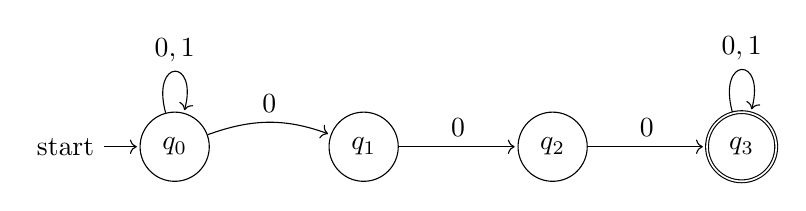
\begin{tikzpicture}[shorten >=1pt,node distance=2.4cm,on grid,auto]
    \node[state,initial] (q0) {$q_0$};
    \node[state] (q1) [right=of q0] {$q_1$};
    \node[state] (q2) [right=of q1] {$q_2$};
    \node[state,accepting] (q3) [right=of q2] {$q_3$};

    \path[->]
    (q0) edge[loop above] node {$0,1$} ()
         edge[bend left=20] node {$0$} (q1)
    (q1) edge node {$0$} (q2)
    (q2) edge node {$0$} (q3)
    (q3) edge[loop above] node {$0,1$} ();
\end{tikzpicture}
\end{center}

Formally,
\[
N_a=(\{q_0,q_1,q_2,q_3\},\{0,1\},\delta,q_0,\{q_3\}),
\]
where
\[
\delta(q_0,0)=\{q_0,q_1\}, \qquad \delta(q_0,1)=\{q_0\},
\]
\[
\delta(q_1,0)=\{q_2\}, \qquad \delta(q_2,0)=\{q_3\},
\]
\[
\delta(q_3,0)=\{q_3\}, \qquad \delta(q_3,1)=\{q_3\},
\]
and all unspecified transitions go to \(\varnothing\).

\subsubsection*{Step 4: Why this works}

\begin{itemize}[itemsep=0.4em]
    \item The loop at \(q_0\) on \(0\) and \(1\) allows the machine to ignore any prefix before the desired substring appears.
    \item On a \(0\), the machine may also branch from \(q_0\) to \(q_1\), meaning ``maybe this is the start of the three-zero block.''
    \item Moving from \(q_1\) to \(q_2\) means a second consecutive \(0\) was seen.
    \item Moving from \(q_2\) to \(q_3\) means a third consecutive \(0\) was seen, so the substring \(000\) has appeared.
    \item Once in \(q_3\), the machine stays accepting no matter what follows, because the language only asks whether \(000\) appears somewhere.
\end{itemize}

\subsubsection*{Quick test strings}

\[
000,\ 1000,\ 110001,\ 000111 \in L(N_a)
\]
because each contains \(000\).

\[
\varepsilon,\ 0,\ 00,\ 01010 \notin L(N_a)
\]
because none of these contains \(000\).

\subsection*{1.19(b): \((((00)^*(11))\cup 01)^*\)}

\subsubsection*{Step 1: Parse the expression carefully}

This expression is
\[
\big( ((00)^*(11)) \cup 01 \big)^*.
\]

Work from the inside out.

\begin{itemize}[itemsep=0.4em]
    \item \((00)^*\) means ``an even number of \(0\)'s,'' possibly zero of them.\sipser{Def.~1.23, pp.~44--45, and Def.~1.52, pp.~64--65.}
    \item \((00)^*(11)\) therefore means
    \[
    \text{even number of zeros, followed by }11.
    \]
    Examples: \(11\), \(0011\), \(000011\), \dots
    \item Then we take the union with \(01\), so one \emph{block} is either
    \[
    (00)^*11 \quad \text{or} \quad 01.
    \]
    \item Finally, the outside star means we may concatenate any number of such blocks together, including zero blocks.\sipser{Def.~1.23, pp.~44--45.}
\end{itemize}

So the language consists of all strings that can be chopped into blocks where each block is either \(01\) or an even number of zeros followed by \(11\).

\subsubsection*{Step 2: Build one machine for one block, then loop back}

The outer star suggests the machine should return to the start after finishing a valid block.

\begin{center}
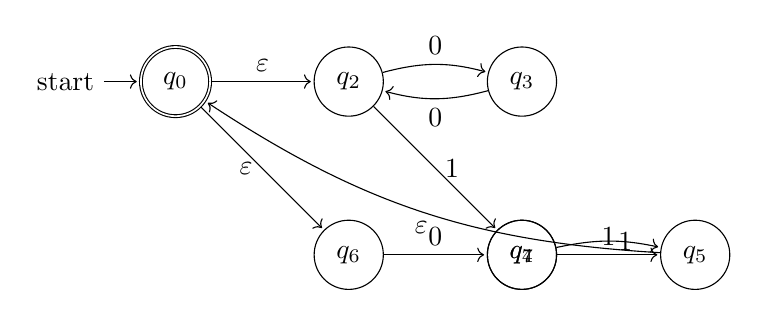
\begin{tikzpicture}[shorten >=1pt,node distance=2.2cm,on grid,auto]
    \node[state,initial,accepting] (q0) {$q_0$};
    \node[state] (q2) [right=of q0] {$q_2$};
    \node[state] (q3) [right=of q2] {$q_3$};
    \node[state] (q4) [below=of q3] {$q_4$};
    \node[state] (q6) [below=of q2] {$q_6$};
    \node[state] (q7) [right=of q6] {$q_7$};
    \node[state] (q5) [right=of q4] {$q_5$};

    \path[->]
    (q0) edge node {$\varepsilon$} (q2)
         edge node[left] {$\varepsilon$} (q6)
    (q2) edge[bend left=15] node {$0$} (q3)
         edge node[right] {$1$} (q4)
    (q3) edge[bend left=15] node {$0$} (q2)
    (q4) edge node {$1$} (q5)
    (q6) edge node {$0$} (q7)
    (q7) edge[bend left=12] node[right] {$1$} (q5)
    (q5) edge[bend left=15] node[below] {$\varepsilon$} (q0);
\end{tikzpicture}
\end{center}

Formally,
\[
N_b=(\{q_0,q_2,q_3,q_4,q_5,q_6,q_7\},\{0,1\},\delta,q_0,\{q_0\}),
\]
where
\[
\delta(q_0,\varepsilon)=\{q_2,q_6\},
\]
\[
\delta(q_2,0)=\{q_3\}, \qquad \delta(q_3,0)=\{q_2\},
\]
\[
\delta(q_2,1)=\{q_4\}, \qquad \delta(q_4,1)=\{q_5\},
\]
\[
\delta(q_6,0)=\{q_7\}, \qquad \delta(q_7,1)=\{q_5\},
\]
\[
\delta(q_5,\varepsilon)=\{q_0\},
\]
and all unspecified transitions go to \(\varnothing\).

\subsubsection*{Step 3: Why this works}

\begin{itemize}[itemsep=0.4em]
    \item From \(q_0\), the machine nondeterministically chooses which kind of block to try by taking an \(\varepsilon\)-move.
    \item The branch through \(q_2,q_3,q_4,q_5\) handles \((00)^*11\):
    \begin{itemize}
        \item \(q_2 \leftrightarrow q_3\) tracks pairs of zeros,
        \item from \(q_2\) a \(1\) means the zero-count is even and we are ready to begin the final \(11\),
        \item \(q_4 \to q_5\) on \(1\) completes that \(11\).
    \end{itemize}
    \item The branch \(q_6 \to q_7 \to q_5\) recognizes the other possible block \(01\).
    \item The \(\varepsilon\)-move from \(q_5\) back to \(q_0\) allows the next block to begin.
    \item The start state \(q_0\) is accepting, so the machine accepts \(\varepsilon\), which it must, because the outer star allows zero blocks.\sipser{Def.~1.23, pp.~44--45.}
\end{itemize}

\subsubsection*{Quick test strings}

\[
\varepsilon,\ 01,\ 11,\ 0011,\ 0111,\ 0101,\ 1101 \in L(N_b)
\]

Explanation:
\begin{itemize}[itemsep=0.3em]
    \item \(\varepsilon\): zero blocks,
    \item \(01\): one \(01\) block,
    \item \(11\): one \((00)^*11\) block with zero zeros,
    \item \(0011\): one \((00)^*11\) block with one pair of zeros,
    \item \(0111 = 01 \cdot 11\),
    \item \(0101 = 01 \cdot 01\),
    \item \(1101 = 11 \cdot 01\).
\end{itemize}

\[
0,\ 1,\ 001,\ 111,\ 0011111 \notin L(N_b)
\]
because they cannot be partitioned into the allowed block types.

\subsection*{1.19(c): \(\varnothing^*\)}

\subsubsection*{Step 1: Translate the expression}

By definition, \(\varnothing\) is the empty language, so it contains no strings at all.\sipser{Def.~1.52, pp.~64--65.}

The star of a language means ``zero or more concatenated strings from that language.''\sipser{Def.~1.23, pp.~44--45.}

If the language is empty, then:
\begin{itemize}[itemsep=0.3em]
    \item no positive-length concatenation is possible, because there are no strings available to choose from,
    \item but the zero-fold concatenation is still allowed, and that gives \(\varepsilon\).
\end{itemize}

Therefore,
\[
\varnothing^*=\{\varepsilon\}.
\]

\subsubsection*{Step 2: Give the NFA}

The language \(\{\varepsilon\}\) is recognized by the one-state NFA whose start state is also accepting.

\begin{center}
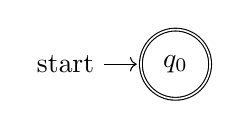
\begin{tikzpicture}[shorten >=1pt,node distance=2cm,on grid,auto]
    \node[state,initial,accepting] (q0) {$q_0$};
\end{tikzpicture}
\end{center}

Formally,
\[
N_c=(\{q_0\},\{0,1\},\delta,q_0,\{q_0\}),
\]
where all transitions go to \(\varnothing\).

\subsubsection*{Step 3: Why this works}

\begin{itemize}[itemsep=0.3em]
    \item If the input is \(\varepsilon\), the machine starts in an accept state and therefore accepts.
    \item If the input contains any symbol at all, there is no transition to follow, so that input is rejected.
\end{itemize}

Thus the machine accepts exactly \(\{\varepsilon\}\), which is exactly \(\varnothing^*\).

\newpage
\section*{Exercise 1.20(e--h)}

These are regular-expression reading exercises. The real task is translating each expression into plain English and then checking whether sample strings fit that description.

Assume
\[
\Sigma=\{a,b\}.
\]
Then \(\Sigma^*\) means all strings made from \(a\) and \(b\), including \(\varepsilon\).\sipser{Ex.~1.51, p.~64.}

\subsection*{1.20(e): \(\Sigma^*a\Sigma^*b\Sigma^*a\Sigma^*\)}

\subsubsection*{Step 1: Read the structure}

This expression says:

\[
\text{anything} \;+\; a \;+\; \text{anything} \;+\; b \;+\; \text{anything} \;+\; a \;+\; \text{anything}.
\]

So the language is:
\[
\{w\in\{a,b\}^* \mid w \text{ contains an } a,\text{ then later a } b,\text{ then later another } a\}.
\]

The three marked symbols do not have to be adjacent. The \(\Sigma^*\) pieces allow arbitrary material between them.

\subsubsection*{Step 2: Give examples}

Members:
\[
aba,\qquad aabba
\]

Why:
\begin{itemize}[itemsep=0.3em]
    \item \(aba\) has exactly the pattern \(a\cdots b\cdots a\).
    \item \(aabba\) has an \(a\), then later a \(b\), then later another \(a\).
\end{itemize}

Nonmembers:
\[
aaa,\qquad bbaab
\]

Why:
\begin{itemize}[itemsep=0.3em]
    \item \(aaa\) contains no \(b\), so the middle requirement fails.
    \item \(bbaab\) does contain \(a\)'s and a \(b\), but after the final \(b\) there is no later \(a\).
\end{itemize}

\subsection*{1.20(f): \(aba \cup bab\)}

\subsubsection*{Step 1: Translate the union}

The union symbol means ``either the left language or the right language.''\sipser{Def.~1.23, pp.~44--45.}

So this language contains exactly the two strings
\[
aba \quad \text{and} \quad bab.
\]

\subsubsection*{Step 2: Give examples}

Members:
\[
aba,\qquad bab
\]

Nonmembers:
\[
ab,\qquad abba
\]

Reason:
\begin{itemize}[itemsep=0.3em]
    \item \(ab\) is too short and is not equal to either listed string.
    \item \(abba\) is also not exactly \(aba\) or \(bab\).
\end{itemize}

\subsection*{1.20(g): \((\varepsilon \cup a)b\)}

\subsubsection*{Step 1: Understand the union inside the parentheses}

The piece
\[
\varepsilon \cup a
\]
means ``either the empty string or the string \(a\).''\sipser{Def.~1.52, pp.~64--65.}

Now concatenate \(b\) to the end:
\[
(\varepsilon \cup a)b = \varepsilon b \cup ab = b \cup ab.
\]

So the language is exactly
\[
\{b,ab\}.
\]

\subsubsection*{Step 2: Give examples}

Members:
\[
b,\qquad ab
\]

Nonmembers:
\[
a,\qquad bb
\]

Reason:
\begin{itemize}[itemsep=0.3em]
    \item \(a\) is missing the final \(b\).
    \item \(bb\) is neither \(b\) nor \(ab\).
\end{itemize}

\subsection*{1.20(h): \((a \cup ba \cup bb)\Sigma^*\)}

\subsubsection*{Step 1: Translate the prefix condition}

The first part says the string must begin with one of:
\[
a,\qquad ba,\qquad bb.
\]

Then \(\Sigma^*\) means anything may follow afterward.

So this language is the set of all strings that start with \(a\), or start with \(ba\), or start with \(bb\).

Equivalently, the only strings \emph{not} in the language are:
\[
\varepsilon \quad \text{and} \quad b.
\]

Why? Because any nonempty string either starts with \(a\) or starts with \(b\). If it starts with \(b\) and has at least one more symbol, then that second symbol is either \(a\) or \(b\), so the string starts with \(ba\) or \(bb\).

\subsubsection*{Step 2: Give examples}

Members:
\[
a,\qquad bbab
\]

Nonmembers:
\[
\varepsilon,\qquad b
\]

Reason:
\begin{itemize}[itemsep=0.3em]
    \item \(a\) starts with \(a\).
    \item \(bbab\) starts with \(bb\).
    \item \(\varepsilon\) has no prefix at all.
    \item \(b\) starts with \(b\), but it is too short to start with \(ba\) or \(bb\).
\end{itemize}

\newpage
\section*{Problem 1.29(b)}

Sipser's Problem 1.29(b) asks for a pumping-lemma proof that
\[
A_2=\{www \mid w\in\{a,b\}^*\}
\]
is not regular.\sipser{Problem 1.29, p.~89; Pumping Lemma, Thm.~1.70, pp.~77--78.}

\subsection*{What the language means}

The notation
\[
\{www \mid w\in\{a,b\}^*\}
\]
means:
\begin{quote}
Take any binary string \(w\) over the alphabet \(\{a,b\}\), and repeat that exact same string three times in a row.
\end{quote}

Examples in the language:
\[
\varepsilon\varepsilon\varepsilon=\varepsilon,\qquad
(a)(a)(a)=aaa,\qquad
(ab)(ab)(ab)=ababab.
\]

Examples not in the language:
\[
aab,\qquad ababba.
\]

The key issue is that the language requires the machine to verify that the \emph{same block} appears three times consecutively.

\subsection*{Proof by contradiction using the pumping lemma}

Assume, for contradiction, that \(A_2\) is regular.\sipser{For the standard contradiction template, see Example 1.73, pp.~80--81.} Then by the pumping lemma, there exists a pumping length \(p\ge 1\) such that every string \(s\in A_2\) with \(|s|\ge p\) can be written as
\[
s=xyz
\]
with
\[
|y|>0,\qquad |xy|\le p,
\]
and
\[
xy^iz\in A_2 \quad \text{for every } i\ge 0.\sipser{Thm.~1.70, pp.~77--78.}
\]

\subsubsection*{Step 1: Choose a string in the language}

Let
\[
s=(a^pb)(a^pb)(a^pb).
\]

This string is in \(A_2\), because if we let
\[
w=a^pb,
\]
then
\[
s=www.
\]

Also, \(|s|\ge p\), so the pumping lemma applies.

\subsubsection*{Step 2: Use the condition \(|xy|\le p\)}

The first \(p\) symbols of \(s\) are all \(a\)'s. Since \(|xy|\le p\), the substring \(y\) lies entirely inside that initial block of \(a\)'s.\sipser{This is exactly the kind of use of condition 3 that Sipser highlights in the pumping lemma statement and follow-up discussion, pp.~77--78 and Example 1.73, pp.~80--81.}

Therefore,
\[
y=a^k
\]
for some integer \(k\ge 1\), because \(|y|>0\).

\subsubsection*{Step 3: Pump once upward}

Take \(i=2\). Then
\[
xy^2z = a^{p+k}ba^pba^pb.
\]

Call this new string \(t\):
\[
t=a^{p+k}ba^pba^pb.
\]

If the pumping lemma were correct for this language, then \(t\) would still have to belong to \(A_2\).

\subsubsection*{Step 4: Show that \(t\notin A_2\)}

Suppose, toward a contradiction, that \(t\in A_2\). Then there exists some string \(u\) such that
\[
t=uuu.
\]

Now count the number of \(b\)'s in \(t\). There are exactly three.

Because \(t\) is the concatenation of three identical copies of \(u\), the number of \(b\)'s in \(u\) must be exactly one. It cannot be \(0\), because then \(t\) would contain no \(b\)'s. It cannot be \(2\) or more, because then \(t\) would contain at least \(6\) \(b\)'s.

So each copy of \(u\) has exactly one \(b\).

Also, the whole string \(t\) ends in \(b\). Since
\[
t=uuu,
\]
the last symbol of \(t\) is the last symbol of \(u\). Therefore \(u\) itself must end in \(b\).

But if \(u\) contains exactly one \(b\) and ends in \(b\), then \(u\) must have the form
\[
u=a^m b
\]
for some \(m\ge 0\).

That means
\[
uuu=(a^mb)(a^mb)(a^mb).
\]

In such a string, the three blocks of consecutive \(a\)'s must all have the same length \(m\).

However,
\[
t=a^{p+k}ba^pba^pb
\]
has three \(a\)-blocks of lengths
\[
p+k,\qquad p,\qquad p.
\]

These are not all equal because \(k\ge 1\). So \(t\) cannot be of the form \(uuu\).

This contradiction shows that
\[
xy^2z\notin A_2.
\]

\subsubsection*{Step 5: Conclude}

We found a string \(s\in A_2\) such that every allowed decomposition \(s=xyz\) has the property that pumping \(y\) upward produces a string not in \(A_2\). That contradicts the pumping lemma.

Therefore the assumption that \(A_2\) is regular is false. Hence
\[
\boxed{A_2 \text{ is not regular.}}
\]

\section*{Closing remark for presentation}

The main conceptual lesson is this:

\begin{itemize}[itemsep=0.4em]
    \item Exercises 1.19 and 1.20 are about \emph{reading} regular expression notation and matching it to a machine or a language description.
    \item Problem 1.29(b) is about a \emph{limitation} of finite automata: they cannot generally enforce a threefold exact copy condition such as \(www\).
\end{itemize}

That is exactly the transition Sipser makes in Chapter 1: first learning how regular languages work, then learning where they fail.\sipser{Ch.~1 overview: regular expressions, NFAs, and then nonregular languages, pp.~31--89.}

\end{document}
